\subsection{Task 1: Business Ecosystems}
\label{sec:task1}

A business ecosystem is a community of firms that ``coevolve capabilities
around a new innovation'', working both cooperatively and competitively
\parencite[p.~46]{overby2021}. In the digital economy, it describes the
relations and dependencies between digital services, infrastructures, markets
and authorities \parencite[p.~48]{overby2021}. Following \textcite{adner2017},
we start from the value proposition rather than from one firm: cloud services
built on Google technology, run under French control and approved for
sensitive data. The ecosystem consists of the actors that must work together
for this proposition to hold.

Figure~\ref{fig:ecosystem} maps this ecosystem. The blue box is the alliance.
Inside it, Thales owns and controls S3NS, shown by the plain line between them.
S3NS runs PREMI3NS in France, while Google Cloud supplies the underlying
technology, such as computing, storage and data analytics
\parencite{s3ns2025premi3ns}. The grey boxes below are the direct stakeholders.
Client institutions are the customers: around thirty early users, among them
MGEN, Matmut, Club Med and Birdz, while EDF has announced that it has selected
S3NS and Thales itself is a user \parencite{s3ns2025premi3ns}. ANSSI, the
French cybersecurity agency, granted the SecNumCloud qualification in December
2025, which decides whether the offer can host sensitive data at all
\parencite{s3ns2025premi3ns}. Complementors are consultancies, integrators and
software vendors that help clients move to the platform and offer their own
solutions on it \parencite{s3nsecosystem}. The best-known example is SAP, which
has agreed to run its cloud ERP on PREMI3NS \parencite{thalessap2026}.

The orange boxes are indirect stakeholders, which shape the ecosystem without
trading on it. Their influence is shown with dashed arrows. The French state and
US authorities both point at the alliance, because their laws set the
conditions it works under. Under the SREN law and its 2026 decree,
administrations holding particularly sensitive data must use a cloud service
qualified by ANSSI or certified at EU level \parencite{decretsren2026}. The US
CLOUD Act lets US authorities demand data from US providers even when it is
stored abroad \parencite{doj2019cloudact}, which is the reason a
French-controlled offer is needed in the first place. Competitors such as Bleu,
built by Orange and Capgemini on Microsoft technology \parencite{lemagit2023usf},
are linked to the alliance by a two-way dashed arrow, since competition affects
both sides. End users point to the client institutions rather than to the
alliance, because they reach the platform only through the institutions that
hold their data. As \textcite[p.~58]{overby2021} stress, authorities and
consumers are easy to overlook but can decide a firm's survival.

\begin{figure}[htbp]
    \centering
    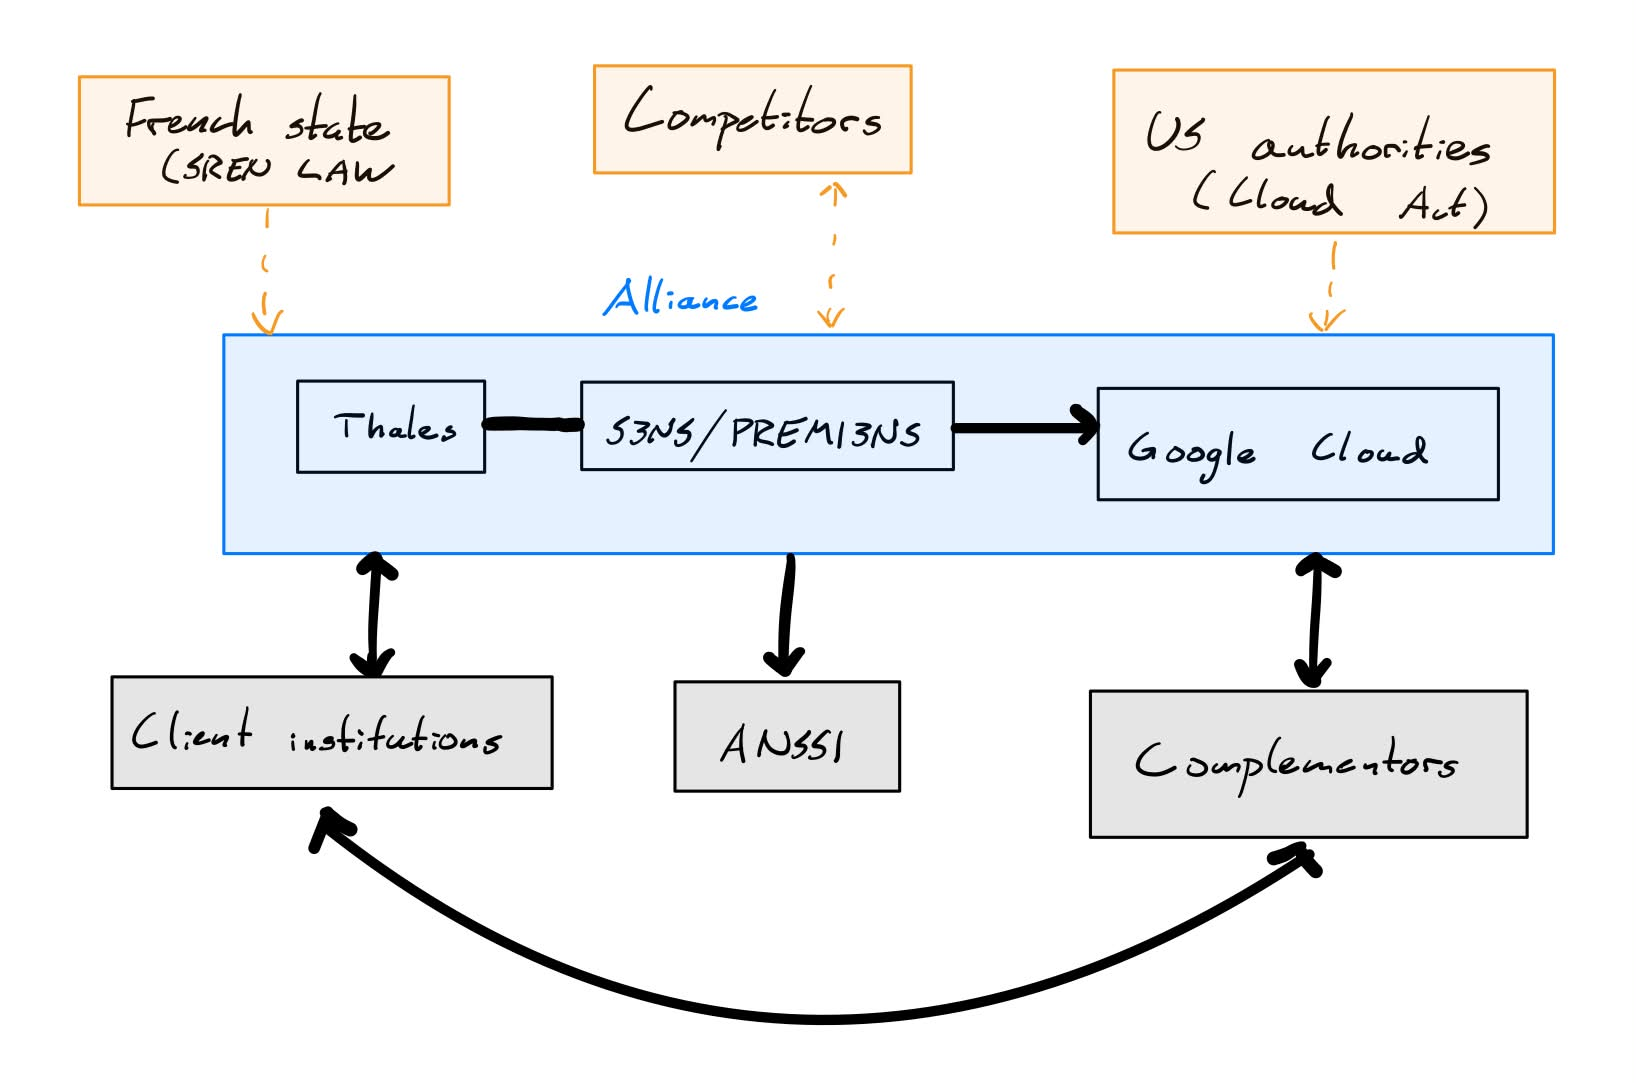
\includegraphics[width=0.85\linewidth]{figures/ecosystem.jpg}
    \caption{Business ecosystem of S3NS. The blue box is the alliance, grey
    boxes are direct stakeholders and orange boxes indirect stakeholders. An
    arrow from A to B means that A depends on B, and a double arrow means mutual
    dependency (notation after \textcite[p.~49]{overby2021}). Dashed arrows show
    indirect influence through law, competition or, for end users, through the
    client institutions. The plain line between Thales and S3NS marks ownership
    and control.}
    \label{fig:ecosystem}
\end{figure}

\subsubsection{Critical relationships and dependencies}

Following the notation of \textcite[p.~49]{overby2021}, a single arrow in
Figure~\ref{fig:ecosystem} shows one-way dependency and a double arrow mutual
dependency. Three of these links are critical.

The first is the single arrow from S3NS to Google Cloud inside the alliance
box. S3NS depends on Google, but Google does not depend on S3NS, so the most
important dependency lies inside the alliance itself. Every Google update first
enters a quarantine zone, where S3NS checks and approves it before it is
deployed in an environment that only S3NS runs \parencite{s3ns2025premi3ns}.
This link carries both the value of the offer, modern cloud services, and its
main risk. Google's technology is closely tied to the service and has no ready
substitute; in course terms it is co-specialised and has low fungibility
\parencite[slide~30]{windekilde2026ecosystem}. S3NS could not switch provider
without rebuilding its service, and clients inherit this dependency through
S3NS, since their systems are built on Google-based services.

The second is the single arrow from the alliance down to ANSSI. The alliance
depends on the qualification, while ANSSI does not depend on the alliance.
This dependency is about regulation rather than technology, but it is just as
critical: without the qualification, the demand created by the SREN law
disappears.

The third is the curved double arrow between client institutions and
complementors. Clients can only move their systems if the software they need
is available on the platform, and vendors only qualify their software if there
are enough clients to sell to. This is why the SAP agreement matters
\parencite{thalessap2026}. The alliance is linked to both groups by double
arrows as well, since it needs their custom and contributions as much as they
need the platform.

\subsubsection{Complementarities}

The partners bring what the other lacks. Google brings technology it has
already built at global scale, while Thales brings French ownership, security
expertise and control. By using Google as its cloud provider, S3NS can offer a
full service without building all the technology itself
\parencite[p.~54]{overby2021}. The complementarity is \emph{unilateral}: S3NS
needs Google's technology to work, but Google's business does not need S3NS
\parencite[p.~114]{overby2021}. This matches the book's example of Skype and
Internet service providers, where Skype needs the providers but not the other
way round \parencite[p.~115]{overby2021}.

PREMI3NS also complements the software of the vendors. For a regulated client,
the platform is worth little unless the applications it needs can run there,
and the software is worth more when it can run inside a qualified cloud. The
complementarity is \emph{supermodular}, meaning that more of one makes the
other more valuable: more qualified software makes PREMI3NS more attractive,
and more PREMI3NS customers make it more worthwhile for vendors to qualify
their software \parencite[slides~27--28]{windekilde2026ecosystem}. This part of
the ecosystem is still small, as the vendor model on PREMI3NS is described as
being at an early stage \parencite{futurum2026}.

\subsubsection{How the alliance changes roles, incentives and influence}

The alliance changes the position of each main actor compared with acting
alone, which is why Thales and Google are drawn inside one box in
Figure~\ref{fig:ecosystem}. Google goes from being a foreign supplier, and a
competitor through its own public cloud, to a technology partner. It reaches
regulated French customers it could not serve directly, but gives up control of
the operation to S3NS. Thales goes from security specialist to cloud owner and
operator, and is also a key customer, both on PREMI3NS and as SAP's first
customer on the platform \parencite{thalessap2026}. The French state goes from
buyer to market creator, since its rules create the demand the alliance serves
\parencite{decretsren2026}. The partners' incentives are not fully aligned:
Thales must guarantee independence, while Google gains from wider use of its
technology, including by repeating the model in Germany
\parencite{thalesgoogle2026}. Influence in the ecosystem therefore rests on a
paradox. Thales holds formal control, but Google holds the technology the whole
ecosystem depends on.